\section{Исследовательская часть}

\subsection{Команды и формат задания правил}
Для того, чтобы посмотреть все команды и формат задаваемых правил, необходимо вызвать \textbf{help}. На Рисунке \ref{fig11:image} представлен результат.

\begin{figure}[h]
	\begin{center}
		{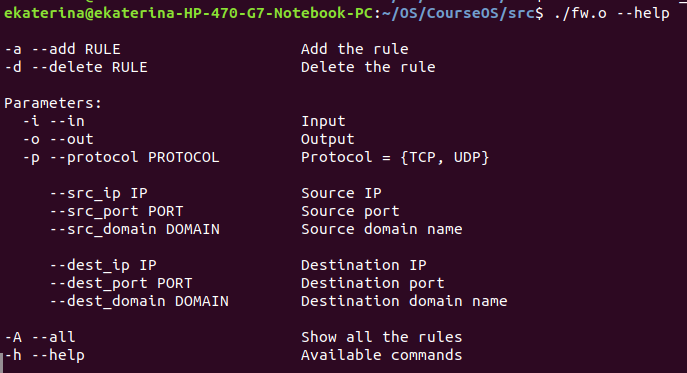
\includegraphics[scale = 0.6]{img/screenshots/help/help.png}}
		\caption{Вызов команды help}
		\label{fig11:image}
	\end{center}
\end{figure}
Для того, чтобы корректно задать правило фильтрации, необходимо соблюдать следующий формат.
\begin{enumerate}
	\item Обязательным является указание действий: добавление (add) или удаление (del).
	
	\item Также в обязательном порядке следует конкретизировать направление пакетов: входящие (in) или исходящие (out).
	
	\item Далее указываются основные признаки фильтрации (один или несколько):
	\begin{itemize}
		\item протокол (TCP/UDP);
		
		\item IP-адрес (источника/назначения);
		
		\item порт (источника/назначения);
		
		\item доменное имя (источника/назначения). \newline
	\end{itemize}
	
\end{enumerate}

\subsection{Видимость модуля}
Для скрытия модуля следует вызвать команду \textbf{hide}, а для обратного действия \textbf{unhide}. На Рисунках \ref{fig40:image} -- \ref{fig41:image} демонстрируется следующее:
\begin{enumerate}
	\item модуль загружен и виден в системе;
	
	\item вызвана команда hide;
	
	\item модуль не отображается при вызове команды lsmod;
	
	\item вызвана команда unhide;
	
	\item модуль обнаруживается при вызове команды lsmod.
\end{enumerate}

\begin{figure}[h]
	\begin{center}
		{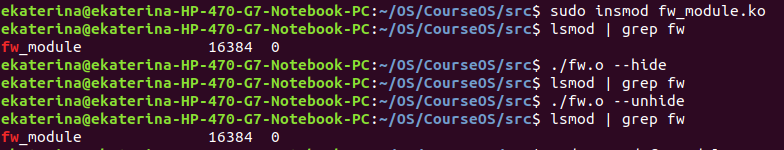
\includegraphics[scale = 0.6]{img/screenshots/hide_unhide/hide_comm.png}}
		\caption{Порядок действий}
		\label{fig40:image}
	\end{center}
\end{figure}

\begin{figure}[h]
	\begin{center}
		{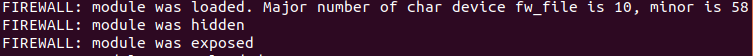
\includegraphics[scale = 0.7]{img/screenshots/hide_unhide/hide_result.png}}
		\caption{Логи}
		\label{fig41:image}
	\end{center}
\end{figure}

\subsection{Фильтрация по протоколу}
Для наглядности было добавлено правило, блокирующее все входящие пакеты, для передачи которых используется протокол TCP.

До того, как правило было добавлено, наблюдалась следующая динамика (Рисунок \ref{fig42:image}): происходил активный обмен пакетами, ошибки в процессе были, но не значительные.
\begin{figure}[h]
	\begin{center}
		{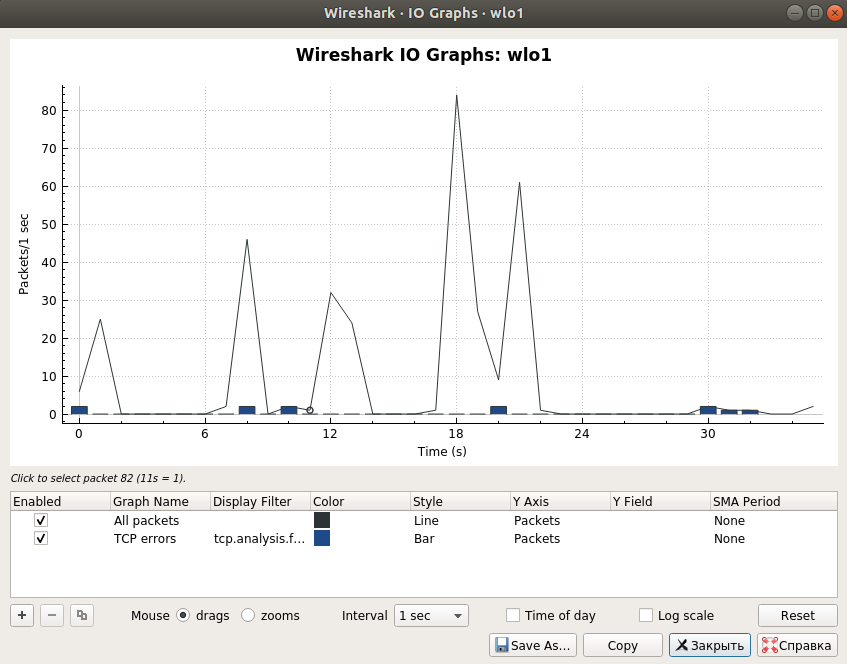
\includegraphics[scale = 0.5]{img/screenshots/rule_protocol/1_rule_protocol.png}}
		\caption{До добавления правила фильтрации}
		\label{fig42:image}
	\end{center}
\end{figure}

\newpage

Когда же правило было зарегистрировано, ситуация изменилась (Рисунок \ref{fig43:image}). Примерно с 50 секунды наблюдается увеличение непринятых пакетов, более детальную информацию о них можно получить из log-файла (Рисунок \ref{fig44:image}). Легко заметить, что общее у всех непринятых пакетов -- поле протокола. 
\begin{figure}[h]
	\begin{center}
		{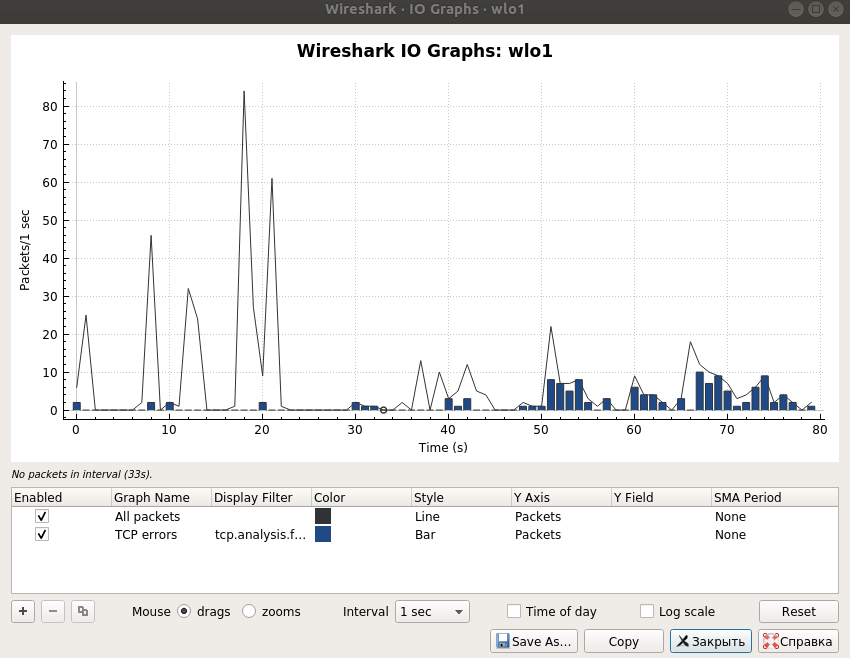
\includegraphics[scale = 0.5]{img/screenshots/rule_protocol/2_rule_protocol.png}}
		\caption{После добавления правила фильтрации}
		\label{fig43:image}
	\end{center}
\end{figure}

\begin{figure}[h]
	\begin{center}
		{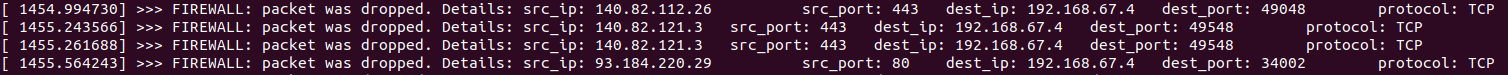
\includegraphics[scale = 0.6]{img/screenshots/rule_protocol/log_drop_packets.png}}
		\caption{Подробная информация о заблокированных пакетах}
		\label{fig44:image}
	\end{center}
\end{figure}

\newpage

При удалении правила, пакеты больше не блокируются, и это видно на Рисунке \ref{fig45:image}.
\begin{figure}[h!]
	\begin{center}
		{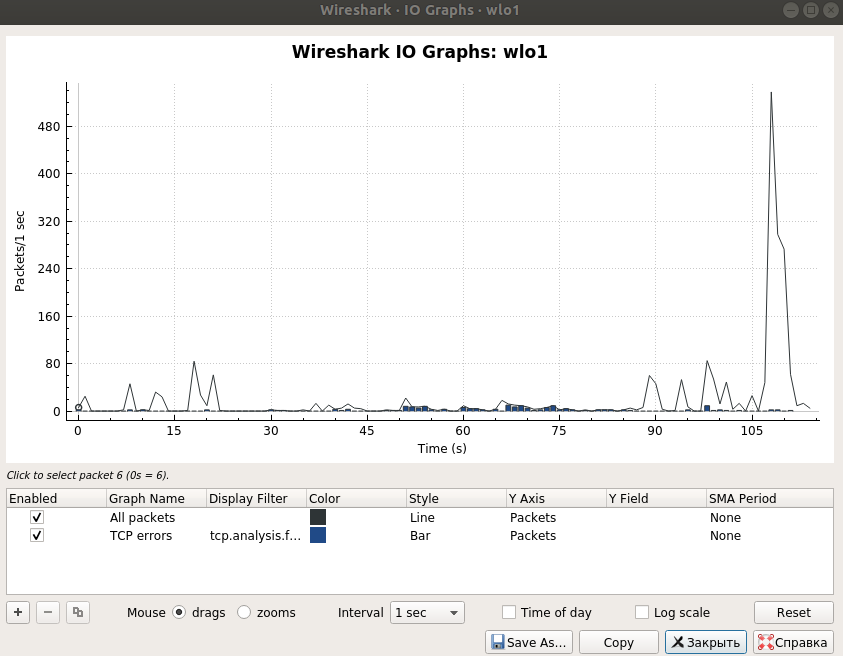
\includegraphics[scale = 0.5]{img/screenshots/rule_protocol/3_rule_protocol.png}}
		\caption{После удаления правила фильтрации}
		\label{fig45:image}
	\end{center}
\end{figure}

\newpage

С 80 секунды наблюдается резкое уменьшение ошибок и увеличение успешно обработанных пакетов. \newline

\subsection{Фильтрация по IP-адресу}
Модуль также предоставляет возможность отбора пакетов по IP-адресу получателя (в случае исходящих пакетов) и отправителя (входящие). 

Было добавлено следующее правило (Рисунок \ref{fig46:image}) и через некоторое время удалено (Рисунок \ref{fig47:image}). 

\begin{figure}[h]
	\begin{center}
		{
\includegraphics[scale = 0.6]{img/screenshots/ip/add_rule.png}}
		\caption{Добавление правила фильтрации по IP-адресу}
		\label{fig46:image}
	\end{center}
\end{figure}

\begin{figure}[h]
	\begin{center}
		{
\includegraphics[scale = 0.6]{img/screenshots/ip/del_rule.png}}
		\caption{Удаление правила фильтрации по IP-адресу}
		\label{fig47:image}
	\end{center}
\end{figure}

\newpage

Устройство, имеющее IP-адрес 192.168.67.132, и устройство, на котором работает межсетевой экран находятся в одной подсети. Поэтому можно с помощью команды \textbf{ping} проверить соединение.

Рисунок \ref{fig48:image} -- результат. Первые 5 и последние 6 пакетов успешно были отправлены в силу того, что правило ещё не было задано или уже удалено на момент их отправки.
\begin{figure}[h]
	\begin{center}
		{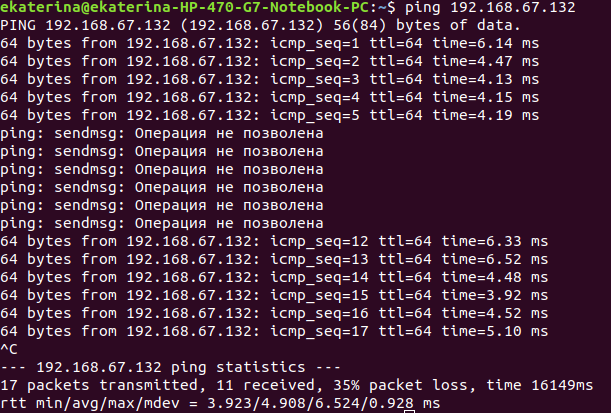
\includegraphics[scale = 0.5]{img/screenshots/ip/result.png}}
		\caption{Результат}
		\label{fig48:image}
	\end{center}
\end{figure}
